\chapter{Supplementary material}

\section{SCI index}
The Social Connectedness Index (SCI) is based on aggregated, anonymized data from Facebook friendship links as of April 2016. It is built from the connections between Facebook users, reflecting the extent of social ties within and between U.S. counties and foreign countries. As of September 2014, over $58\%$ of U.S. adults and $71\%$ of U.S. internet users were on Facebook. Usage was fairly consistent across income, education, and racial groups but declined with age, from $87\%$ among 18-29 year-olds to $56\%$ for those over 65.

In the U.S., Facebook serves primarily as a platform for real-world friends to interact, with individuals typically connecting only with people they know personally. Friendship links on Facebook require mutual consent, and the total number of friends a person can have is capped at $5,000$. This makes Facebook an effective tool for representing U.S. friendship networks on a large scale. The SCI is constructed by mapping Facebook users to their county and country locations, based on profile data and activity, and measuring the total number of friendship links between these regions. Only friendship links among Facebook users who have interacted with Facebook over the 30 days prior to the April 2016 snapshot are considered. The SCI is normalized to a maximum value of 1,000,000, with Los Angeles County having the highest value due to its dense network of local connections.

\section{Data preparation and integration}
 Initially, I merged two datasets, which I will refer to as \textit{Dataset 1} \cite{ChuckConnellFIPS2County} and \textit{Dataset 2} \cite{RussellSamoraGist}, to create a comprehensive table of county-level data. \textit{Dataset 1} contains the names of the counties and their associated states, while \textit{Dataset 2} provides the positions (latitude and longitude) of each county. After merging the datasets, I manually added the missing values from either of the two to ensure all relevant information was available. These datasets are crucial for ensuring the completeness of the analysis.

Next, I compared the merged dataset with the county\_county dataset, which was obtained from \textit{The Humanitarian Data} Exchange site \cite{HUMDataSocialConnectedness}. To further refine the data, I identified and added counties that were missing from the first two datasets.

The final dataset was manipulated to focus on county-level SCI flows. First, I kept only the rows where the origin and destination countries matched, then I excluded same-county SCI flows. Then, I created a graph for each country.

To evaluate the elasticity, I had to introduce another dataset, called \textit{Population}, obtained from the \textit{American Community Survey (ACS)}, with population data of American counties from $2017$  to $2021$ \cite{USCensusACS2021}. Some countries were missing from this dataset but they were composed of $2-3$ nodes so they were not included in the analysis.

\section{SCI considerations}

The topographical map of Pennsylvania \ref{fig:Top_Penn} alongside the corresponding Social Connectedness Index (SCI) network \ref{fig:SCI_filt_Penn} illustrate the high SCI values observed in counties within the Appalachian Mountains.
\begin{figure}[ht]
    \centering
    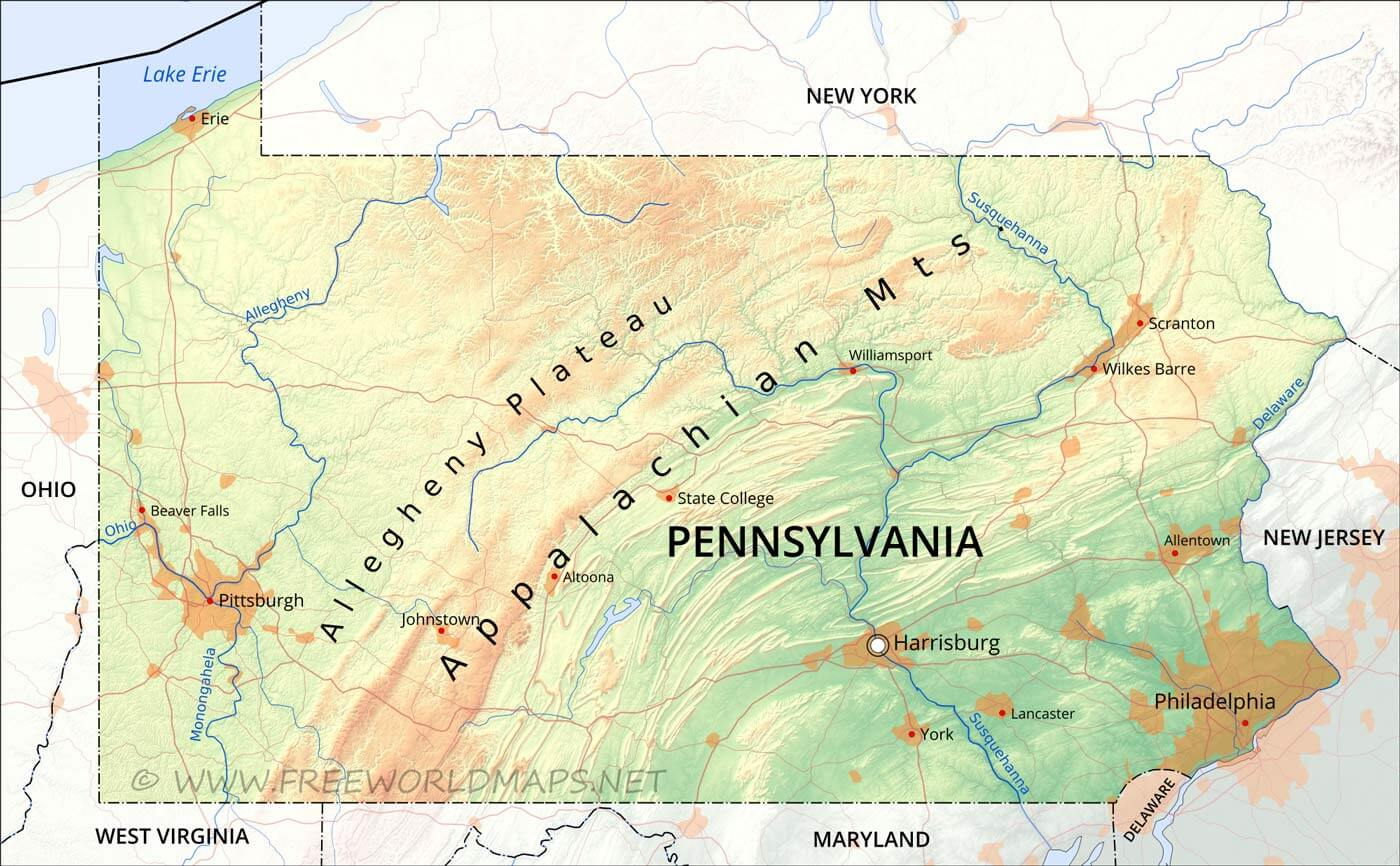
\includegraphics[width=0.7\linewidth]{images/pennsylvania-map.jpg}
    \caption{Topographical Map of Pennsylvania}
    \label{fig:Top_Penn}
\end{figure}
\begin{figure}[ht]
    \centering
    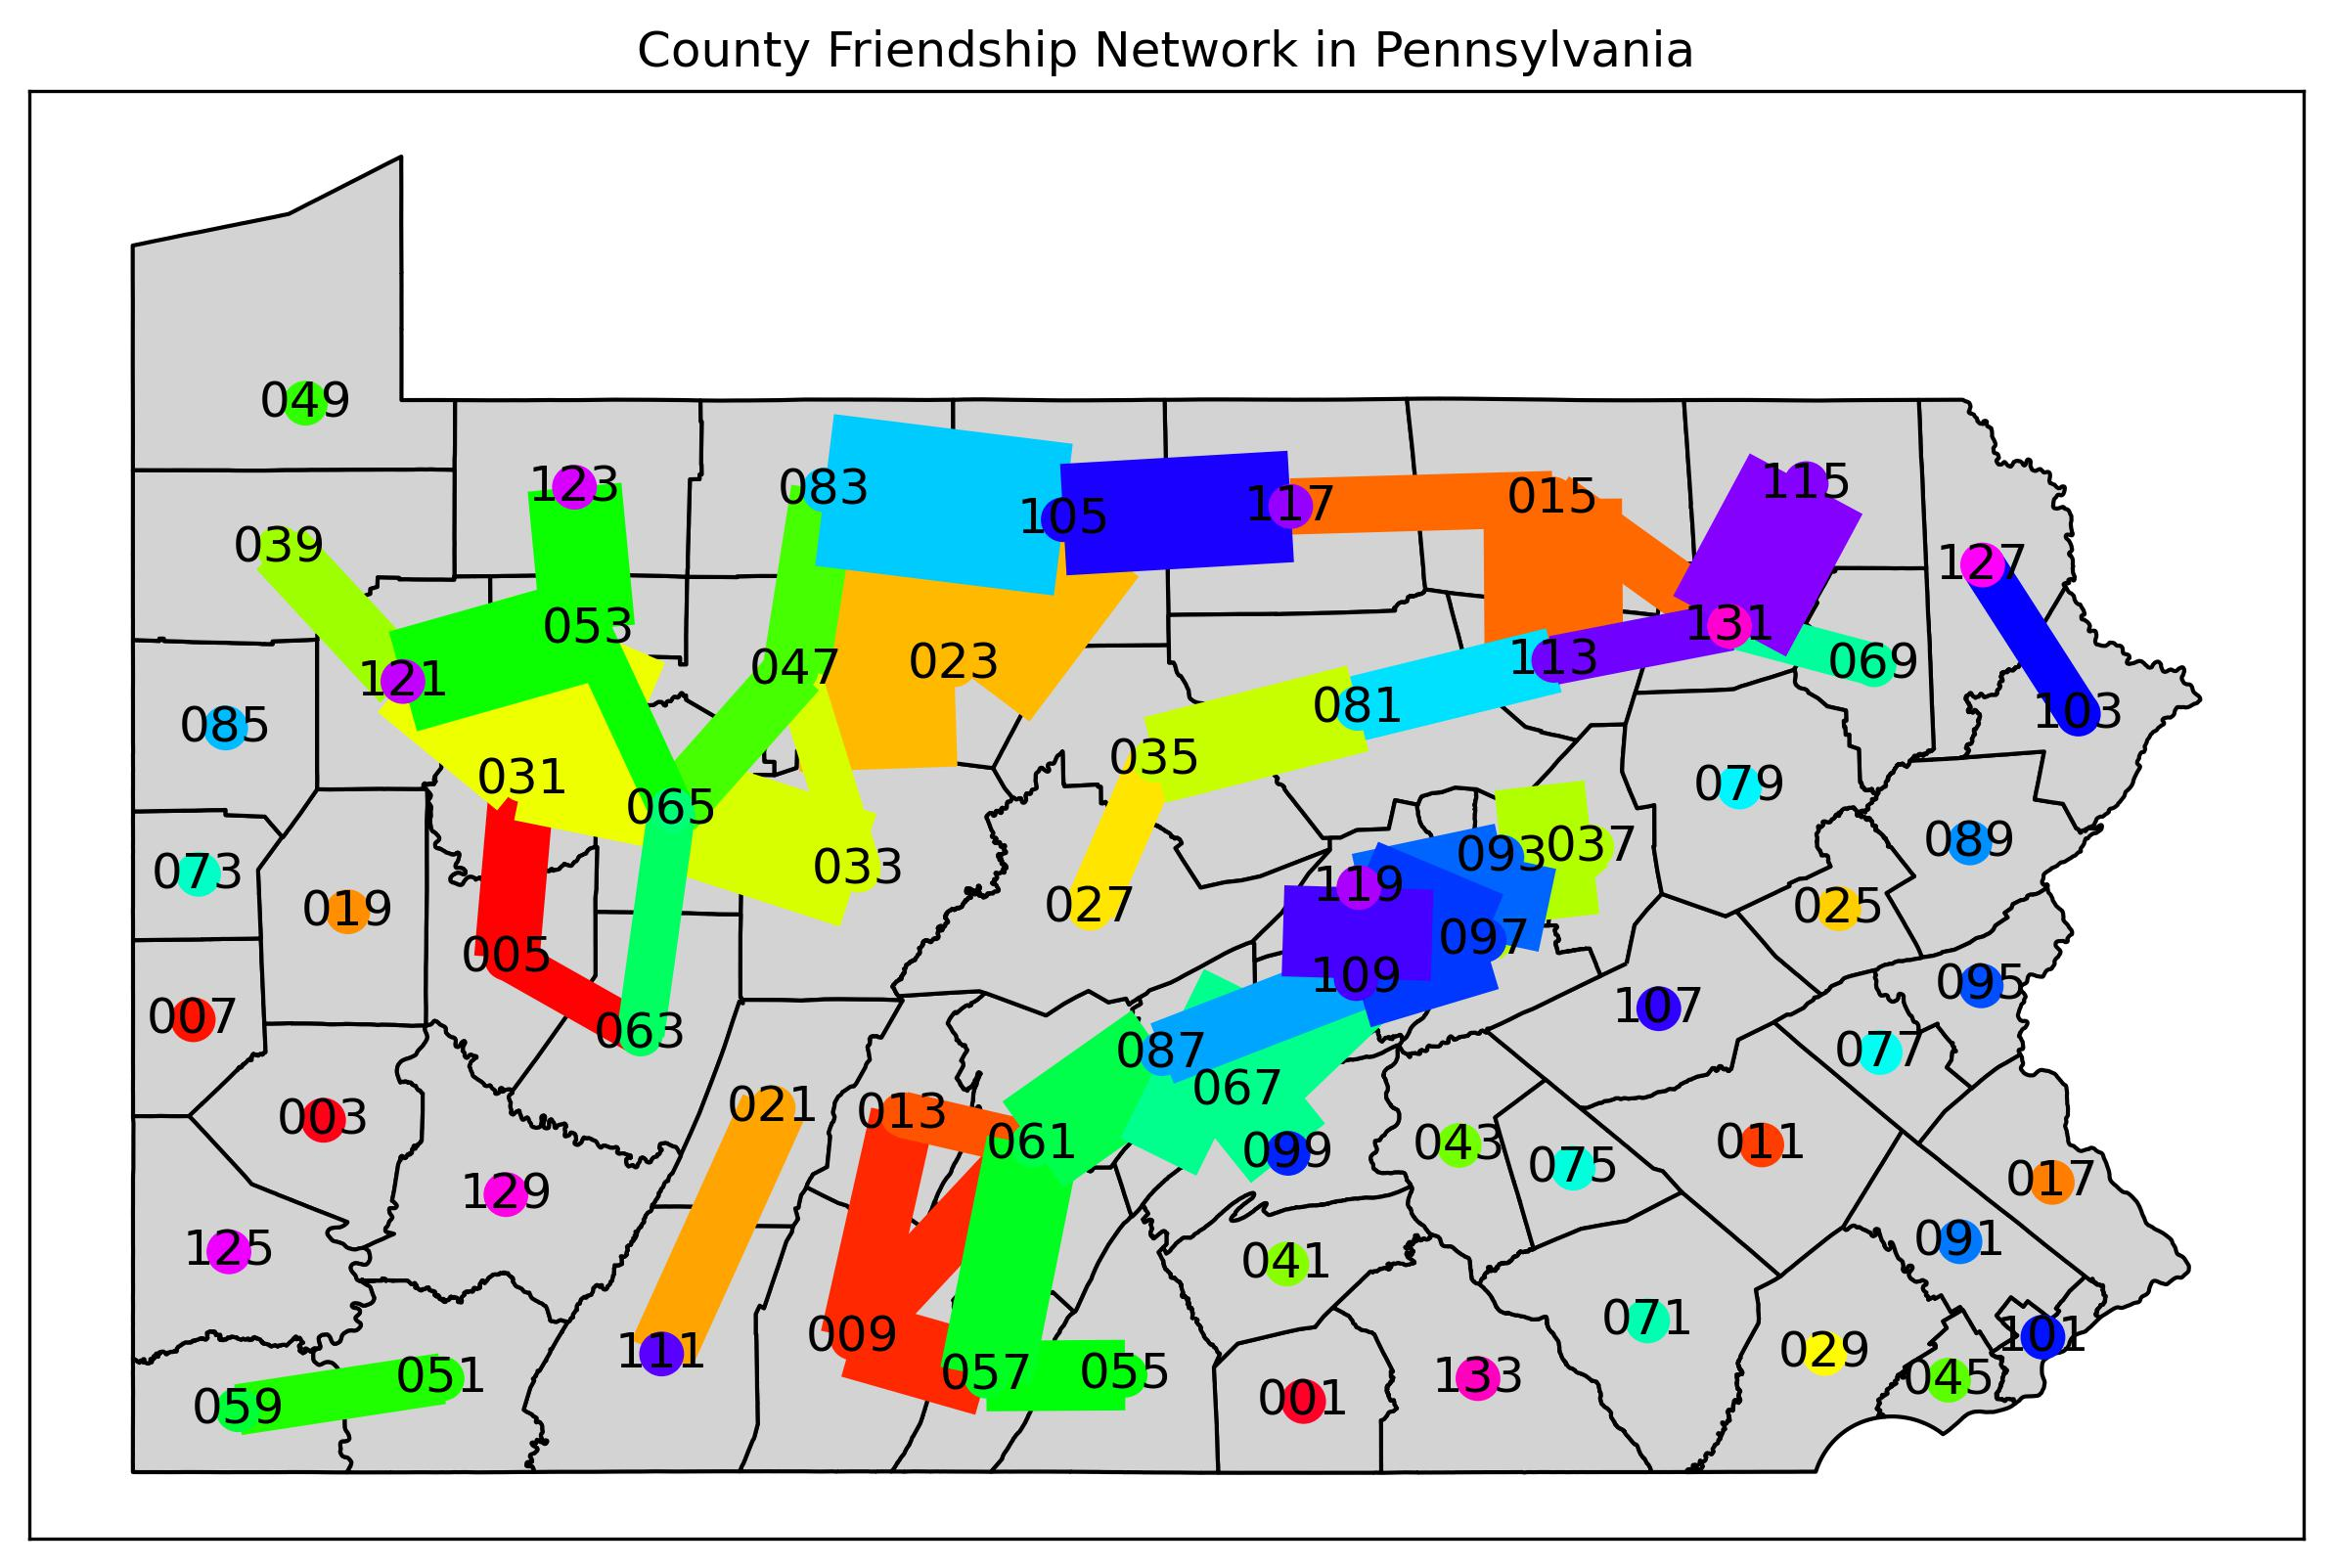
\includegraphics[width=0.7\linewidth]{images/network_filtered_Pennsylvania.jpg}
    \caption{Pennsylvania SCI map where edges with SCI smaller than 20\% of the maximum SCI value in the country have been removed, to enhance clarity }
    \label{fig:SCI_filt_Penn}
\end{figure}

In \ref{fig:SCI-Flo}, on the other hand, the SCI map of Florida where migration patterns caused strong connections to non-adjacent northern regions but low SCI values inside the country.

\begin{figure}[ht]
    \centering
    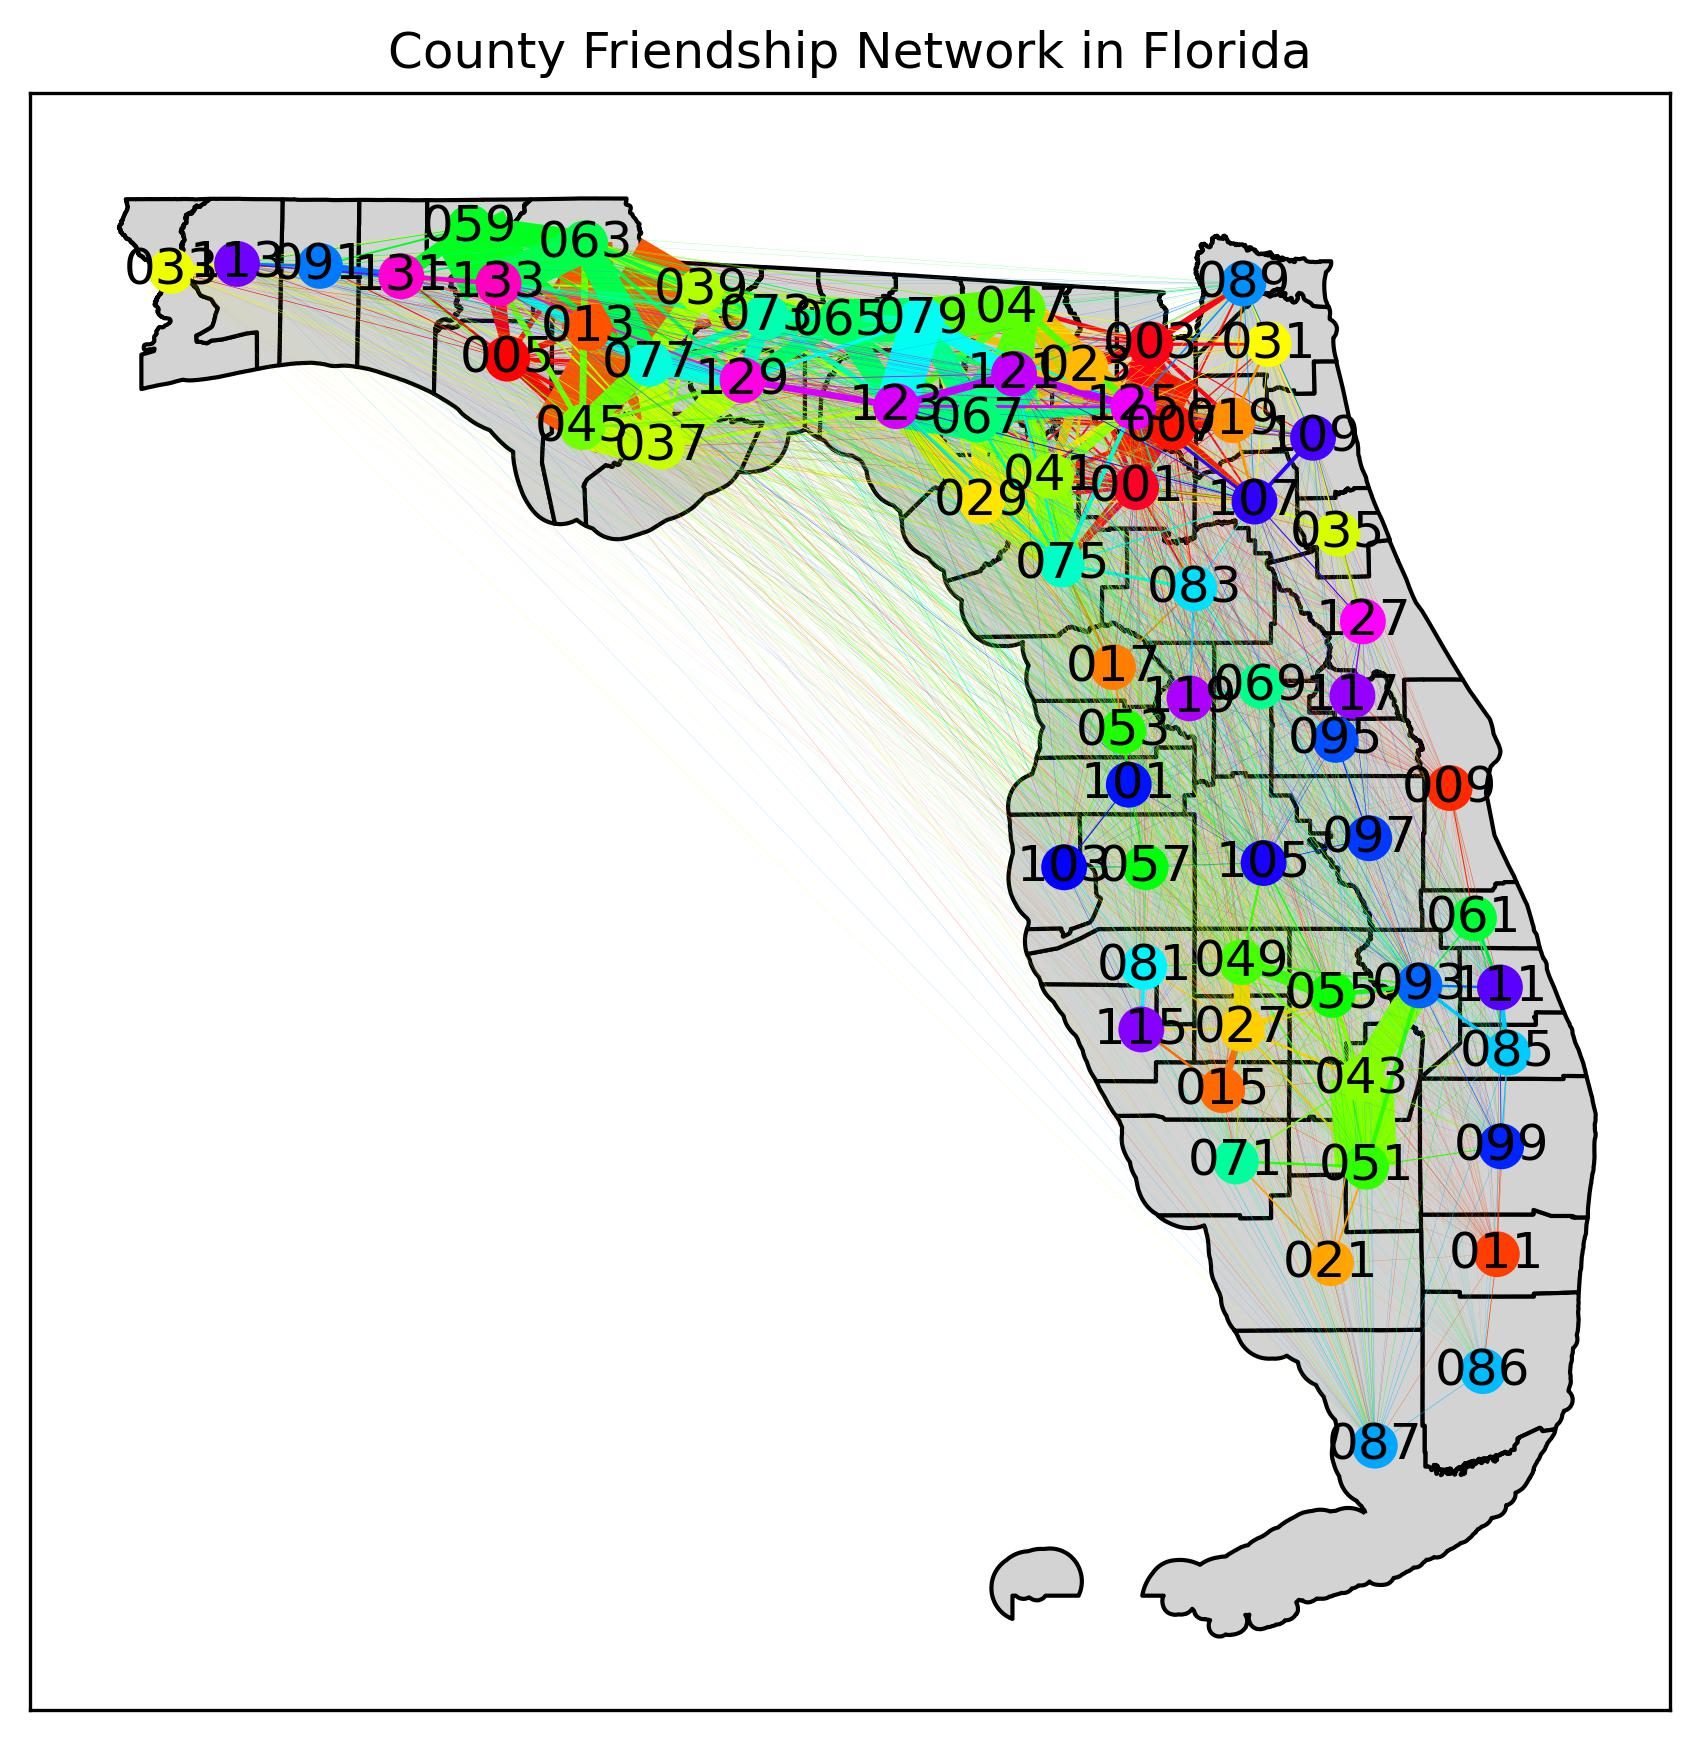
\includegraphics[width=0.7\linewidth]{images/network_Florida.jpg}
    \caption{Florida SCI map}
    \label{fig:SCI-Flo}
\end{figure}

\section{Elasticity}

Table \ref{tab:elasticity_results} shows the regression coefficients for states with more than 50 counties, ensuring a more reliable fit for the elasticity model. The coefficients are reported for three models: $\beta_1^{\text{all}}$, $\beta_1^{\text{lt}}$ (short distances, less than $200 \ miles$), and $\beta_1^{\text{ge}}$ (long distances, more than $200 \ miles$ ).

The results align with Bailey et al.'s findings, showing that elasticity is more negative for short distances, indicating a steeper decline in social connectedness as distance increases. For example, Alabama shows a sharp decrease in short-distance elasticity $(-2.57)$, which then flattens at longer distances $(-1.19)$.

The variation across states may reflect differences in migration, local culture, or infrastructure. In Florida, for instance, the elasticity for short distances is quite negative $(-2.47)$, which could suggest that local ties are weakened by long-distance connections, as already mentioned. This idea could be further explored by examining migration patterns in more detail.

\begin{table}[H]
    \centering
    \begin{tabular}{lccc}
        \hline
        State & $\beta_1^{\text{all}}$ & $\beta_1^{\text{lt}}$ & $\beta_1^{\text{ge}}$ \\
        \hline
        Alabama & -2.15 $\pm$ 0.02 & -2.573 $\pm$ 0.03 & -1.19 $\pm$ 0.06 \\
        Arkansas & -2.03 $\pm$ 0.01 & -2.31 $\pm$ 0.03 & -1.59 $\pm$ 0.05 \\
        California & -1.17 $\pm$ 0.02 & -1.59 $\pm$ 0.07 & -1.12 $\pm$ 0.03 \\
        Colorado & -1.29 $\pm$ 0.03 & -1.74 $\pm$ 0.07 & -0.70 $\pm$ 0.06 \\
        Florida & -1.46 $\pm$ 0.02 & -2.47 $\pm$ 0.05 & -0.93 $\pm$ 0.03 \\
        Georgia & -1.89 $\pm$ 0.01 & -2.26 $\pm$ 0.02 & -1.34 $\pm$ 0.02 \\
        Illinois & -2.22 $\pm$ 0.01 & -2.64 $\pm$ 0.02 & -1.75 $\pm$ 0.03 \\
        Indiana & -2.05 $\pm$ 0.01 & -2.37 $\pm$ 0.01 & -1.65 $\pm$ 0.04 \\
        Iowa & -1.99 $\pm$ 0.01 & -2.25 $\pm$ 0.01 & -1.91 $\pm$ 0.03 \\
        Kansas & -1.61 $\pm$ 0.01 & -1.98 $\pm$ 0.04 & -1.40 $\pm$ 0.03 \\
        Kentucky & -2.01 $\pm$ 0.01 & -2.35 $\pm$ 0.01 & -1.40 $\pm$ 0.02 \\
        Louisiana & -1.96 $\pm$ 0.02 & -2.22 $\pm$ 0.03 & -1.47 $\pm$ 0.04 \\
        Michigan & -1.30 $\pm$ 0.01 & -1.98 $\pm$ 0.03 & -0.85 $\pm$ 0.03 \\
        Minnesota & -1.47 $\pm$ 0.01 & -1.92 $\pm$ 0.03 & -1.05 $\pm$ 0.03 \\
        Mississippi & -2.09 $\pm$ 0.01 & -2.38 $\pm$ 0.02 & -1.80 $\pm$ 0.04 \\
        Missouri & -2.14 $\pm$ 0.01 & -2.50 $\pm$ 0.02 & -1.87 $\pm$ 0.02 \\
        Montana & -1.33 $\pm$ 0.02 & -1.6 $\pm$ 0.1 & -1.18 $\pm$ 0.04 \\
        Nebraska & -1.45 $\pm$ 0.02 & -1.71 $\pm$ 0.04 & -1.51 $\pm$ 0.04 \\
        New York & -1.90 $\pm$ 0.10 & -1.77 $\pm$ 0.04 & -2.13 $\pm$ 0.07 \\
        North Carolina & -1.65 $\pm$ 0.05 & -2.26 $\pm$ 0.02 & -1.05 $\pm$ 0.02 \\
        North Dakota & -1.67 $\pm$ 0.10 & -2.09 $\pm$ 0.04 & -1.38 $\pm$ 0.05 \\
        Ohio & -2.17 $\pm$ 0.05 & -2.41 $\pm$ 0.02 & -1.80 $\pm$ 0.04 \\
        Oklahoma & -1.57 $\pm$ 0.08 & -2.09 $\pm$ 0.03 & -0.90 $\pm$ 0.03 \\
        Pennsylvania & -2.14 $\pm$ 0.07 & -2.25 $\pm$ 0.03 & -2.10 $\pm$ 0.04 \\
        South Dakota & -1.5 $\pm$ 0.1 & -1.68 $\pm$ 0.04 & -1.41 $\pm$ 0.05 \\
        Tennessee & -1.95 $\pm$ 0.05 & -2.48 $\pm$ 0.02 & -1.40 $\pm$ 0.02 \\
        Texas & -1.74 $\pm$ 0.04 & -2.17 $\pm$ 0.03 & -1.62 $\pm$ 0.01 \\
        Virginia & -1.73 $\pm$ 0.04 & -1.94 $\pm$ 0.02 & -1.40 $\pm$ 0.02 \\
        West Virginia & -2.11 $\pm$ 0.07 & -2.22 $\pm$ 0.02 & -2.22 $\pm$ 0.09 \\
        Wisconsin & -1.66 $\pm$ 0.07 & -1.97 $\pm$ 0.03 & -1.28 $\pm$ 0.04 \\
        \hline
    \end{tabular}
    \caption{Regression Coefficients for States with more than 50 counties}
    \label{tab:elasticity_results}
\end{table}

\section{Modularity}

Building on our previous discussion, intriguing spatial patterns emerge when examining community modules in relation to geographic features. For example, in Montana \ref{fig:Montana_modularity} the map reveals distinct clusters: green dots indicate counties associated with the Rocky Mountain regions, while blue dots represent counties in the northern part of the river.
\begin{figure}
    \centering
    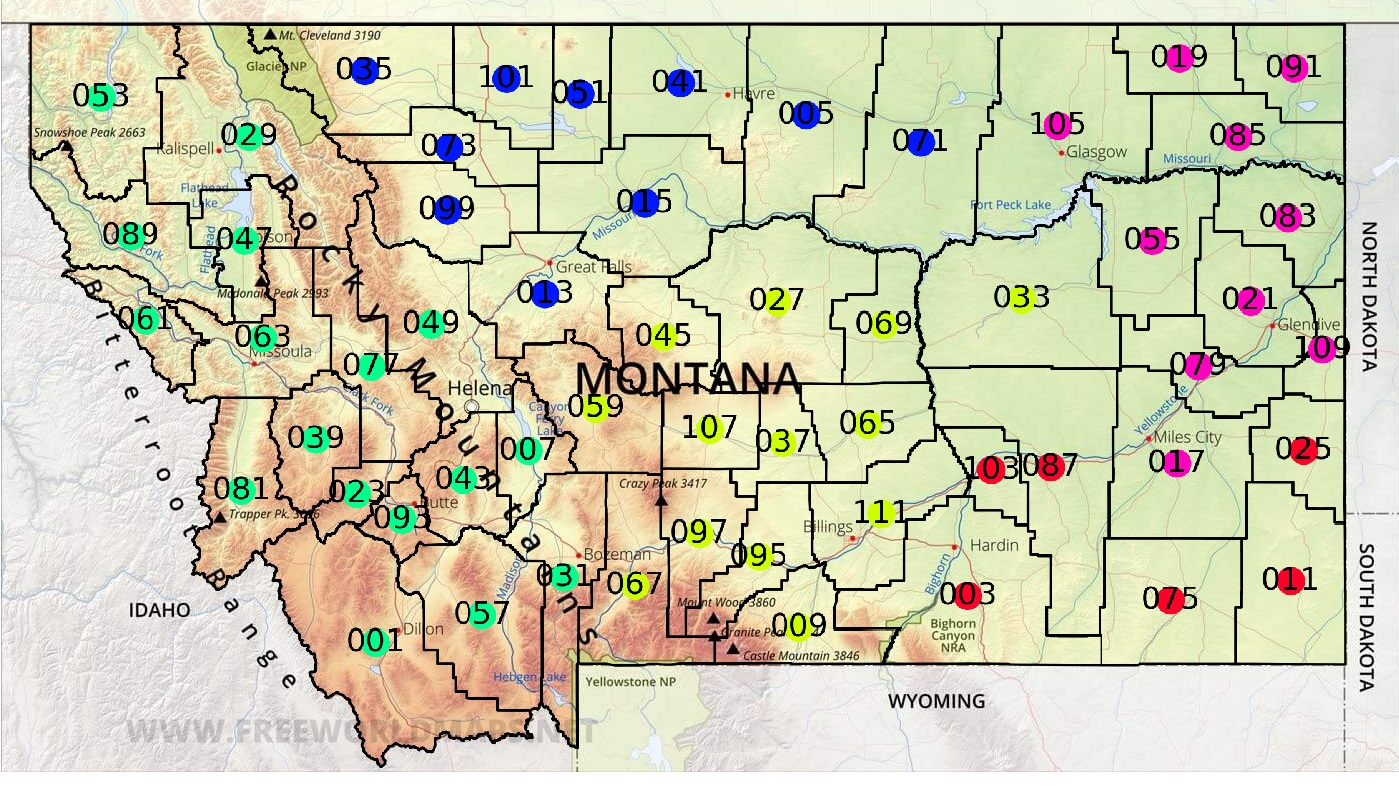
\includegraphics[width=\linewidth]{images/montana_superimposed.jpg}
    \caption{Topographical map of Montana and modules found via Louvain algorithm}
    \label{fig:Montana_modularity}
\end{figure}

A similar pattern is observed in other states along the Rocky Mountains, such as Colorado, as well as in the Appalachian region, including Georgia, suggesting that natural geographic barriers play a key role in shaping social connectivity.

Beyond geography, modularity patterns may also reflect urban-rural divisions, economic dependencies, and historical migration trends, which could be explored in future research.

\section{Use of ChatGPT}

In this project, ChatGPT \cite{OpenAI2025} primarily assisted with the superimposition plot of the network and U.S. counties, including the automatic generation of the plot and the implementation of saving functions for the obtained results. It also contributed to locating some datasets, such as U.S. FIPS codes and population data, though further evaluation was required on my part to identify the most complete and reliable sources. Additionally, ChatGPT played a role in the final revision of the review, refining my initial draft to enhance clarity, professionalism, and appropriateness of language.


\newpage